\section{Scalability}

\subsection{Question (Paper \& Pencil)}     % subsection 1.1

\subsubsection{Constant input $x_o$ and threshold $\theta^*$}       % subsubsection 1.1.1
In the case of constant input and constant threshold ($x(t)=x_o$ and $\theta(t) = \theta^*$), the BCM learning rule has the form: 
\begin{equation}
\frac{d\omega_i}{dt} = \eta x_i(y^2-y\theta)= Aw^2-Bw
\end{equation}
where A and B are constants. Here, the main problem of this learning rule would be that the weights grow without bound, so they can not converge to stable values.  
\subsubsection{Stability of fixed points}
For the coupled differential equations: 

\begin{eqnarray}
\tau \dot \theta_M &=&  -\theta_M + y^p \\
\dot \omega &=& \eta x (y^2-y\theta) \\
\end{eqnarray}

we assume $\tau << \eta^{-1}$, so we can assume that $\theta$ converges much faster than $\omega$. At a fixed point for p=0, we would have: 

\begin{eqnarray}
\tau \dot \theta_M &=&  -\theta_M + y^p \\
0 &=& -\theta_M + y^p \\
\theta_M &=& 1
\end{eqnarray}
and 
\begin{eqnarray}
\dot \omega &=& \eta x (y^2-y) \\
\dot \omega &=& \eta x^2 \omega (\omega x- 1) \label{eq:p0}
\end{eqnarray}

so the fixed points are at $\omega = 0$ and $\omega = 1/x$. Fig. \ref{fig:p0} shows the plot of $\dot \omega$ for p=0, with the only stable fixed point being $\omega = 0$. 

\begin{figure}[h]
\centering
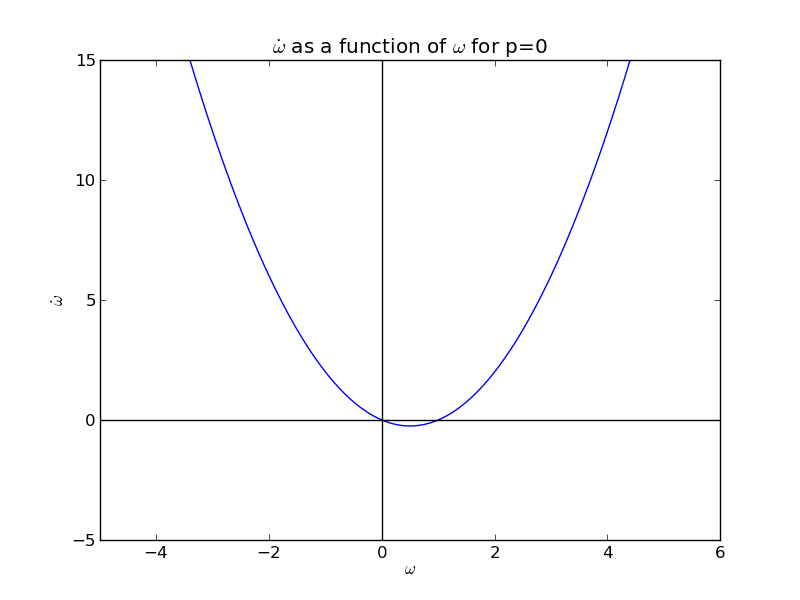
\includegraphics[width=0.7\textwidth]{./p0.png}
\caption{Fixed points of $\dot \omega$ are $\omega = 0$ and $\omega = 1/x$, as shown in figure. (Eq. \ref{eq:p0}). For simplicity we assume x=1.}
\label{fig:p0}
\end{figure}

For p=1, the coupled ODE's look like: 

\begin{eqnarray}
\tau \dot \theta_M &=&  -\theta_M + y \\
\theta_M &=& y
\end{eqnarray}
which leads to
\begin{eqnarray}
\dot \omega &=& \eta x (y^2-y^2) \\
\dot \omega &=& 0 \label{eq:p1}
\end{eqnarray}

and since the Eq. \ref{eq:p1} is zero everywhere, the system has either already converged or it is trivial, so we cannot discuss its stability as a function of $\omega$.

For p=2, the coupled ODE's are: 

\begin{eqnarray}
\theta_M &=& y^2
\end{eqnarray}

which leads to
\begin{eqnarray}
\dot \omega &=& \eta x (y^2-y^3) \\
\dot \omega &=&  \eta x^3w^2(1-wx) \label{eq:p2}
\end{eqnarray}

so the fixed points are at $\omega = 0$ and $\omega = 1/x$ once again. The only stable fixed point is $\omega = 1/x$ in this case, as can be seen from Fig. \ref{fig:p2}. 

\begin{figure}[h]
\centering
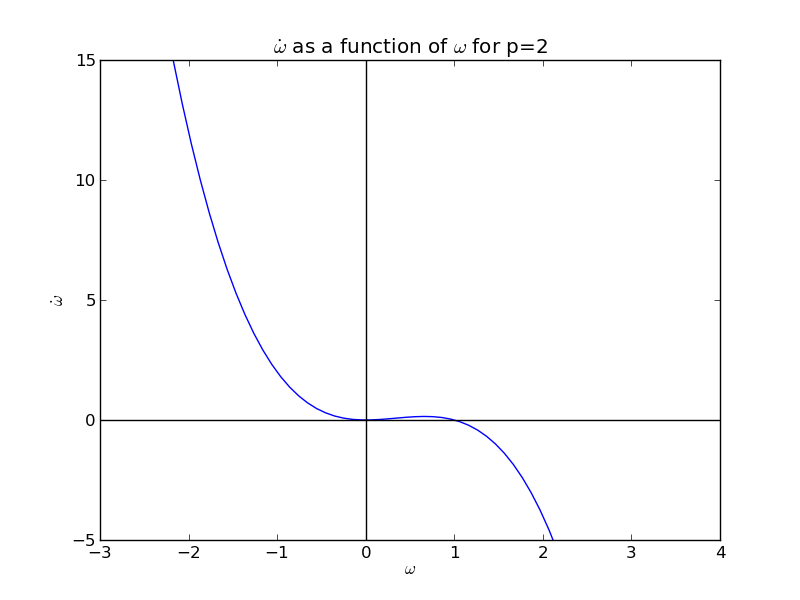
\includegraphics[width=0.7\textwidth]{./p2.png}
\caption{Fixed points of $\dot \omega$ are $\omega = 0$ and $\omega = 1/x$, as shown in figure. (Eq. \ref{eq:p2}, x=1).}
\label{fig:p2}
\end{figure}

For p=3, the coupled ODE's are: 

\begin{eqnarray}
\theta_M &=& y^3
\end{eqnarray}

which leads to
\begin{eqnarray}
\dot \omega &=& \eta x (y^2-y^4) \\
\dot \omega &=&  \eta x^3w^2(1-x^2w^2) \label{eq:p3}
\end{eqnarray}

so the fixed points are at $\omega = 0$ and $\omega = \pm 1/x$. The only stable fixed point is $\omega = 1/x$ again, seen in Fig. \ref{fig:p3}.

\begin{figure}[h]
\centering
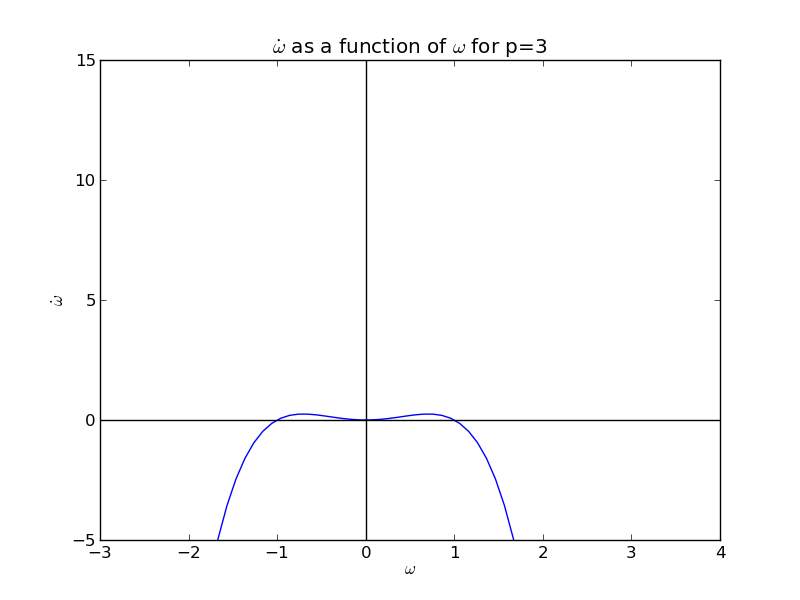
\includegraphics[width=0.7\textwidth]{./p3.png}
\caption{Fixed points of $\dot \omega$ are $\omega = 0$ and $\omega = \pm 1/x$, as shown in figure. (Eq. \ref{eq:p3}, x=1).}
\label{fig:p3}
\end{figure}
\newpage
For p=4, the coupled ODE's are: 

\begin{eqnarray}
\theta_M &=& y^4
\end{eqnarray}

which leads to
\begin{eqnarray}
\dot \omega &=& \eta x (y^2-y^5) \\
\dot \omega &=&  \eta x^3w^2(1-x^3w^3) \label{eq:p4}
\end{eqnarray}

so the fixed points are at $\omega = 0$ and $\omega =  1/x$. Fig. \ref{fig:p4} shows the stability of fixed points for this system, where the only stable fixed point is $\omega = 1/x$ once again.

\begin{figure}[h]
\centering
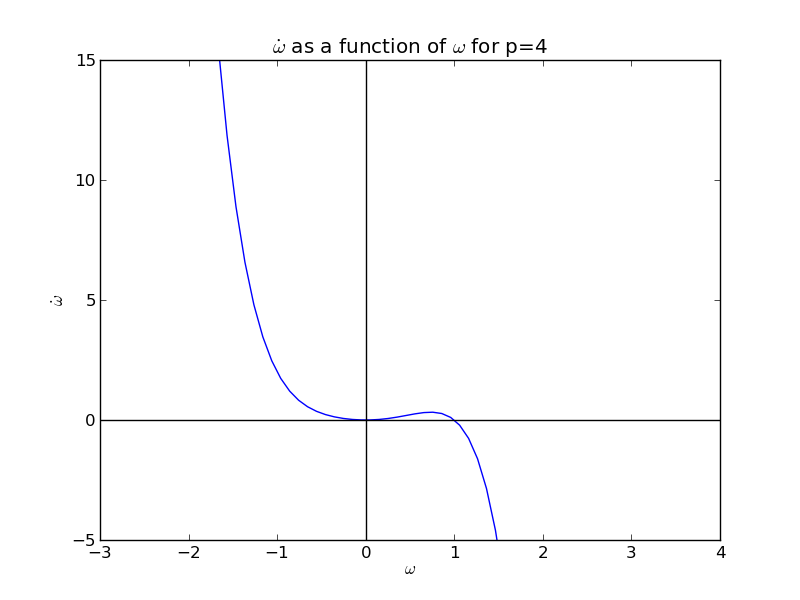
\includegraphics[width=0.7\textwidth]{./p4.png}
\caption{Fixed points of $\dot \omega$ are $\omega = 0$ and $\omega =  1/x$, as shown in figure. (Eq. \ref{eq:p4}, x=1).}
\label{fig:p4}
\end{figure}

We notice from the above examples that we can generalize stability of the fixed points for any $\theta_M = y^p$:
\begin{eqnarray}
\dot \omega &=& \eta x (y^2-y^{p+1}) \\
\dot \omega &=&  \eta x(x^2w^2-x^{p+1}w^{p+1}) \label{eq:general1}
\end{eqnarray}

and taking the derivative of $\dot \omega$ with respect to $\omega$ yields
\begin{eqnarray}
\frac{d\dot \omega}{d\omega} &=& \eta x (2x^2\omega-(p+1)x^{p+1}\omega^p) \label{eq:stab}
\end{eqnarray}

we know that the stability condition for fixed points should satisfy $\frac{d\dot \omega}{d\omega} <0$, so we can see from Eq. \ref{eq:stab} that when  $\omega = 1/x$:
\begin{eqnarray}
\frac{d\dot \omega}{d\omega} &=& \eta x (2x-(p+1)x)  \label{eq:ome}
\end{eqnarray}

and Eq. \ref{eq:ome} is always less than zero for $p > 1$. However, for $\omega = 0$ we see that $\frac{d\dot \omega}{d\omega} <0$ (Eq. \ref{eq:stab}) holds only if p =0. 

Finally, $\omega = -1/x$ can satisfy the stability criteria $\frac{d\dot \omega}{d\omega} <0$ for $p < 1$, but it is not a fixed point for these p values.
